\documentclass[runningheads]{llncs}
\usepackage[T1]{fontenc}

\usepackage[table]{xcolor}

\usepackage{booktabs}
\usepackage[pdfstartview=XYZ,
bookmarks=true,
colorlinks=true,
linkcolor=blue,
urlcolor=blue,
citecolor=blue,
pdftex,
bookmarks=true,
linktocpage=true, % makes the page number as hyperlink in table of content
hyperindex=true
]{hyperref}

\usepackage{rotating} % Rotating table
\usepackage{subcaption}
\usepackage{graphicx}
\usepackage{multirow}
\usepackage{amsmath}
\usepackage{array} % necessary for word wrap within a table



\title{Buyer Beware: Understanding the trade-off between utility and risk in CART based models using simulation data}
\titlerunning{Buyer Beware}

\author{Jonathan Latner\inst{1}\orcidID{0000-0002-1825-0097} \and
Marcel Neunhoeffer\inst{1,2}\orcidID{0000-0002-9137-5785}  \and
J\"{o}rg Drechsler\inst{1,2,3}\orcidID{0009-0009-5790-3394}}

\authorrunning{Latner et al.}


\institute{Institute for Employment Research, Nuremberg, Germany 
\email{\{jonathan.latner, marcel.neunhoeffer,joerg.drechsler\}@iab.de} \and
Ludwig-Maximilians-Universit\"at, Munich, Germany \and
University of Maryland, College Park, USA
}



\begin{document}

\maketitle 

\begin{abstract}

This study examines the trade-off between utility and privacy when generating synthetic data using Classification and Regression Trees (CART) as a Synthetic Data Generator (SDG). Using low-dimensional simulated data with binary variables, we highlight the limitations of CART in mitigating disclosure risks, demonstrate how common privacy metrics do not capture these risks, and propose parameter modifications to balance the trade-off. Our findings underscore the challenges in identifying privacy risks and the necessity of sacrificing utility to enhance privacy, raising critical questions for synthetic data practices.

\keywords{Synthetic data \and Privacy \and CART \and synthpop}
\end{abstract}

\section{Introduction}

The generation of synthetic data has gained prominence as a means to share data while preserving privacy. It is well-established that there is a trade-off between utility and privacy in synthetic data generation \cite{duncan2004database}. CART models, a widely used synthetic data generator (SDG), are noted for their high utility and relatively low privacy risks compared to other methods \cite{little2022comparing,dankar2021fake}. However, the mechanisms that enable CART to minimize this trade-off remain underexplored.

In this paper, we evaluate whether CART-based SDGs effectively mitigate the risk-utility trade-off.  To do so, we borrow from Reiter et al., \cite{reiter2014bayesian} and simulate a low-dimensional data set with 1000 and four binary variables.  Crucially, the last or 1000$^th$ observation is a unique combination of the four binary variables.  In so doing, we create data with an observation we want to protect with synthetic data generated from a CART model.  

In this paper, we seek to make three main contributions.  First, we assess whether we are able to adequately capture the disclosure risks that exist in our simulated data.  Concerns about how to measure utility or privacy in synthetic data are well established.  The problem is not a lack of measures, but rather there is little agreement on which measures are correct for what type of data.  We use common utility and privacy metrics that are available in the Synthpop package \cite{nowok2016synthpop}.  While the results indicate that CART models generate synthetic data with both high levels of utility and privacy, we show that the synthetic data do not protect the disclosive record and this dislosure is not captured by common privacy metrics.  

Second, we explore parameter modifications to the CART-based synthesizer as a potential solution to balance privacy and utility.  On the one hand, we show that one can easily create synthetic data from a CART-based synthesizer that provides a high degree of protection.  On the other hand, we show that one must sacrifice the high levels of utility generated using the default parameters.  Therefore, CART-based synthesizers are capable of generating synthetic data with high levels of privacy protection, but users would have to choose to sacrifice utility even if there is no indication of a disclosure risk.

Third, we propose and evaluate a new implementation of a privacy metric originally developed by Reiter et al., \cite{reiter2014bayesian}. 

<Insert MN text>

In summary, we show that synthetic data from a CART-based SDG are more sensitive to the risk-utility trade-off than was understood from previous research.  Admittedly, we demonstrate this problem using a simulated data set that is unlikely to be used in the real world.  However, the bigger problem is that we demonstrate that a disclosure risk exists in synthetic data that are not captured by common privacy metrics.  If common privacy metrics cannot capture disclosure risks in synthetic data that we know exist (because we created them), then this reduces our confidence that these metrics can capture disclosure risks that we may not know exist.  While we propose solutions to this problem that operate with low-dimensional data, users interested in generating synthetic data should be aware of the challenges we describe here.

\section{Data and Methods}

Following Reiter et al. \cite{reiter2014bayesian}, we simulate one data set with 1.000 observations and four binary categorical variables.  This is our `original' data set.  The first 999 records were sampled from a multinomial distribution for all combinations of var1(0,1), var2(0,1), var3(0,1), var4(0,1), except the last 1000$^th$ record was a unique combination (var1 = 1, var2 = 1, var3 = 1, var4 = 1).  

Figure \ref{fig:frequency} shows the frequency distribution within each of the four variables and figure \ref{fig:histogram} the frequency histogram across all four variables.  They are not evenly distributed within or across the variables because the data are generated from one random sample.  If we were to create 100 samples, then the data would be more even within each of the variables (50\%) and across all four variables (66\%), with the exception of the 1,1,1,1 combination.  However, the critical point is that there is one observation with combination (1,1,1,1) that is not visible if we look at the distribution within each of the variables.

\begin{figure}[!h]
    \centering
    \caption{Original data}
    \begin{subfigure}{0.48\textwidth}
        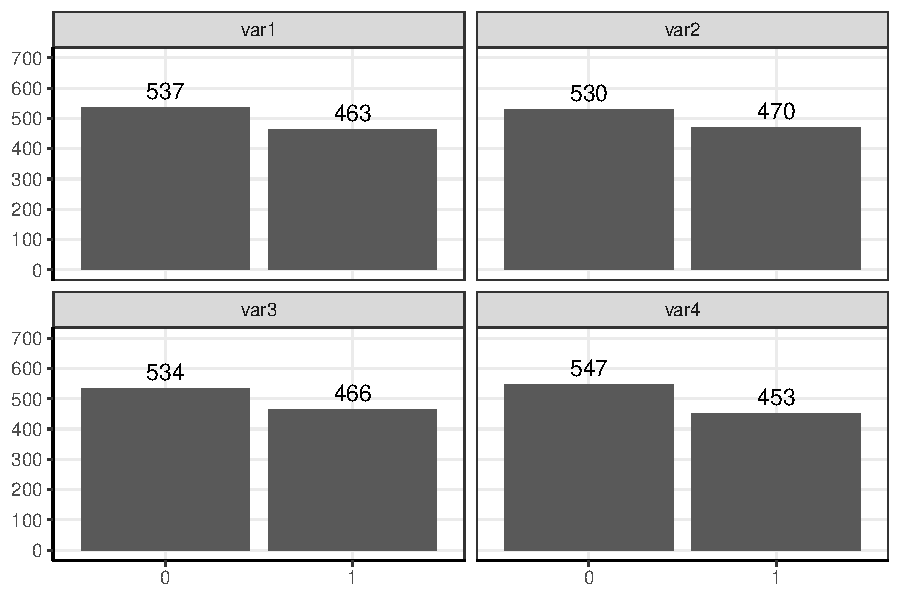
\includegraphics[width=\textwidth]{../graphs/graph_cart_frequency.pdf}
        \caption{Frequency}
        \label{fig:frequency}
    \end{subfigure}
    \hfill
    \begin{subfigure}{0.48\textwidth}
        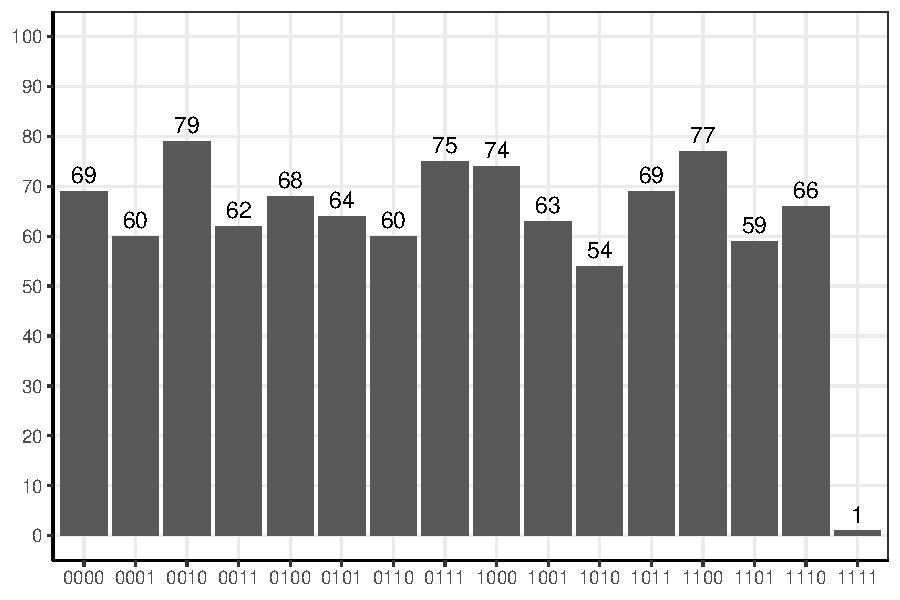
\includegraphics[width=\textwidth]{../graphs/graph_cart_histogram.pdf}
        \caption{Histogram}
        \label{fig:histogram}
    \end{subfigure}
    \label{fig:original}
\end{figure}

Next, we generate one synthetic data from a CART-based SDG from the Synthpop package in R with default parameters (seed=1237).  Figure \ref{fig:frequency_compare} shows the frequency distribution within each of the four variables and figure \ref{fig:histogram_compare} the frequency histogram across all four variables.  Not only do the synthetic data capture the frequency of values within the four variables, but also across all four variables.  The good news is that this means that the synthetic data have high levels of utility.  The bad news is that the synthetic data perfectly replicates the single disclosive record.

\begin{figure}[!h]
    \centering
    \caption{Compare original and synthetic data}
    \begin{subfigure}{0.48\textwidth}
        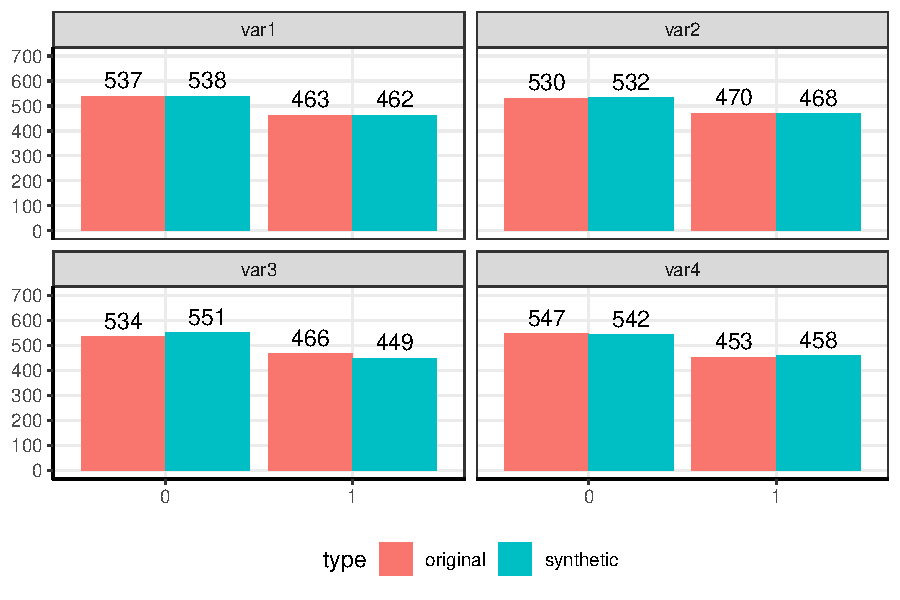
\includegraphics[width=\textwidth]{../graphs/graph_cart_frequency_compare.pdf}
        \caption{Frequency}
        \label{fig:frequency_compare}
    \end{subfigure}
    \hfill
    \begin{subfigure}{0.48\textwidth}
        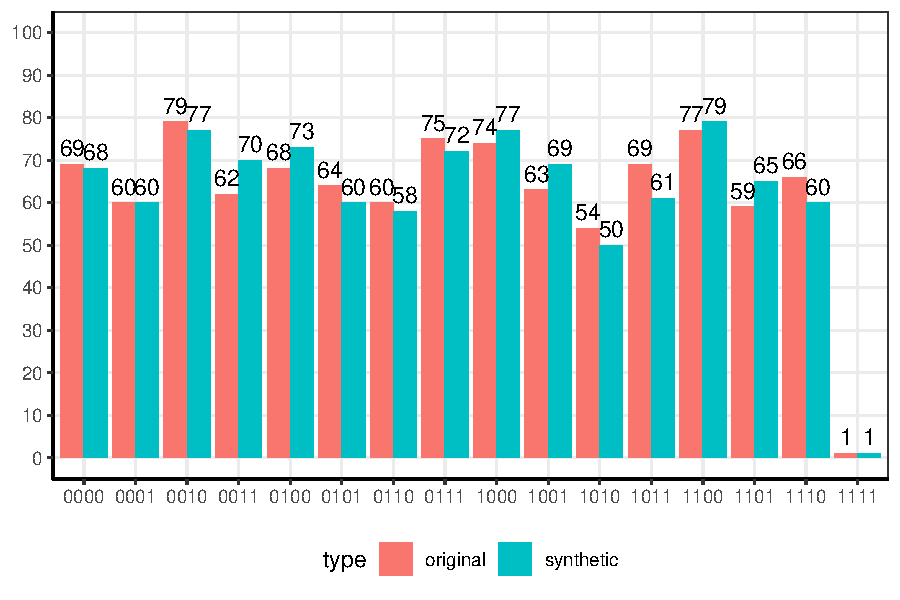
\includegraphics[width=\textwidth]{../graphs/graph_cart_histogram_compare.pdf}
        \caption{Histogram}
        \label{fig:histogram_compare}
    \end{subfigure}
    \label{fig:compare}
\end{figure}

As a sensitivity test, we create 100 synthetic data sets from the original data, as shown in figure \ref{fig:cart_histogram_compare_100}.  Out of 100 synthetic data sets, the frequency of the disclosive record ranges from 0 (41 data sets), 1 (38 data sets), 2 (14 data sets), and 3 (7 data sets).  As a result, regardless of whether one, five, or ten synthetic data sets were released, it would be clear which record was the disclosive record.  As a result, synthetic data from CART models do not protect the unique observation in our simulated data set.  The reason is that in our data with binary categorical data, a record may not be in the synthetic data if it is in the original data, but it can only be in the synthetic data if it is also in the original data.  

\begin{figure}[!h]
    \centering
    \caption{Frequency}
    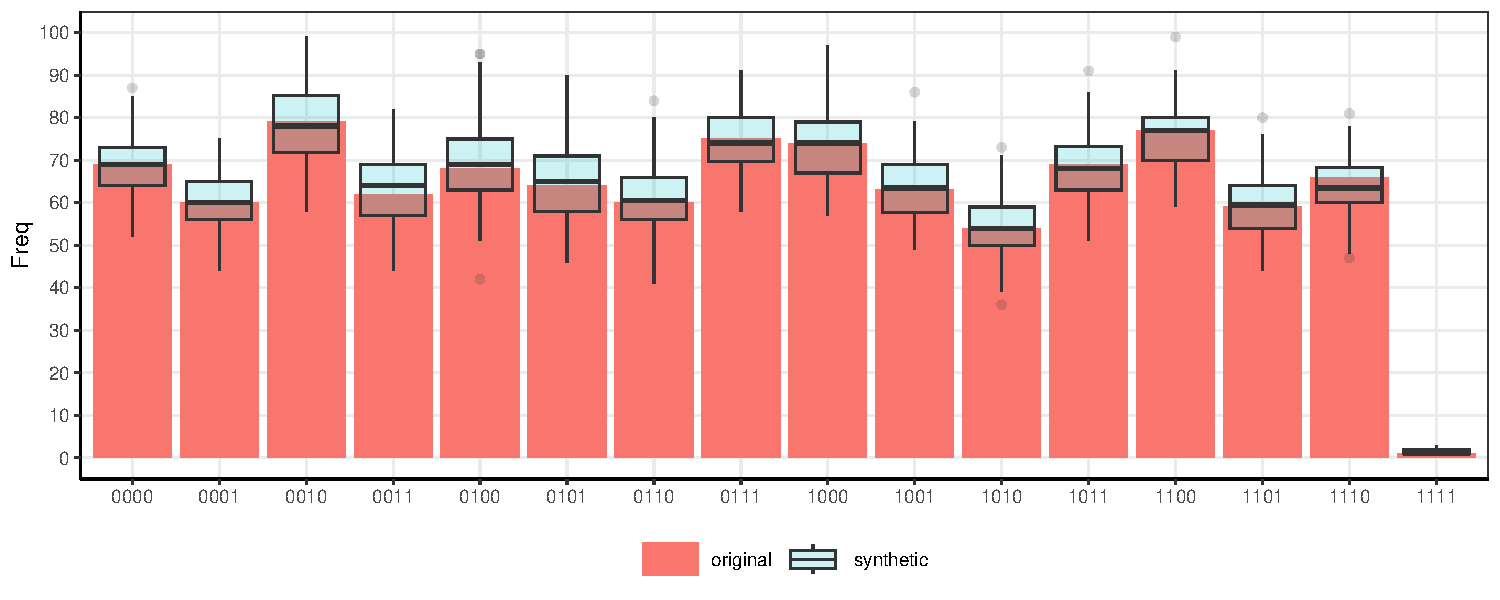
\includegraphics[width=\textwidth]{../graphs/graph_cart_histogram_compare_100.pdf}
    \label{fig:cart_histogram_compare_100}
\end{figure}

\section{The attack}

In this section, we describe an attack scenario.  The basic idea is that an attack is a game between two entities.  On one side, there is a statistical agency who has the data and wants to release it in a privacy preserving way.  On the other side, there is an attacker who wants to identify someone in the data (either membership or attribute inference). The question is what can the attacker learn from a released synthetic data set about an individual they do not have knowledge of?

In this scenario, we assume a `strong' attacker similar to the attack model in differential privacy (DP).  In so doing, we assume that the attacker knows the SDG used to generate the synthetic data.  In our case, this is sequential CART.  They know all observations except the last one.  Further, given the nature of the data, they know all 16 possible combinations that the last record could be.  In this attack, the attacker sees the synthetic data and then runs the same CART-based SDG for each of the 16 different possibilities, sequentially.  Then, they update their beliefs about what the last record could be.

Figure \ref{fig:attacker_default} illustrates the results of this attack with each attack using 100 synthetic data sets.  In the top left cell, the attacker guesses that the last record in the original data is 0,0,0,0.  They then generate 100 synthetic data sets using a CART-based SDG and compare the histogram to the released synthetic data, as shown in figure \ref{fig:compare}.  Remember, the released synthetic data replicates the single unique record found in the original data (1,1,1,1).  

\begin{figure}[!h]
    \centering
    \caption{Histogram of 16 worlds x 100 synthetic datasets}
    \resizebox{\textwidth}{!}{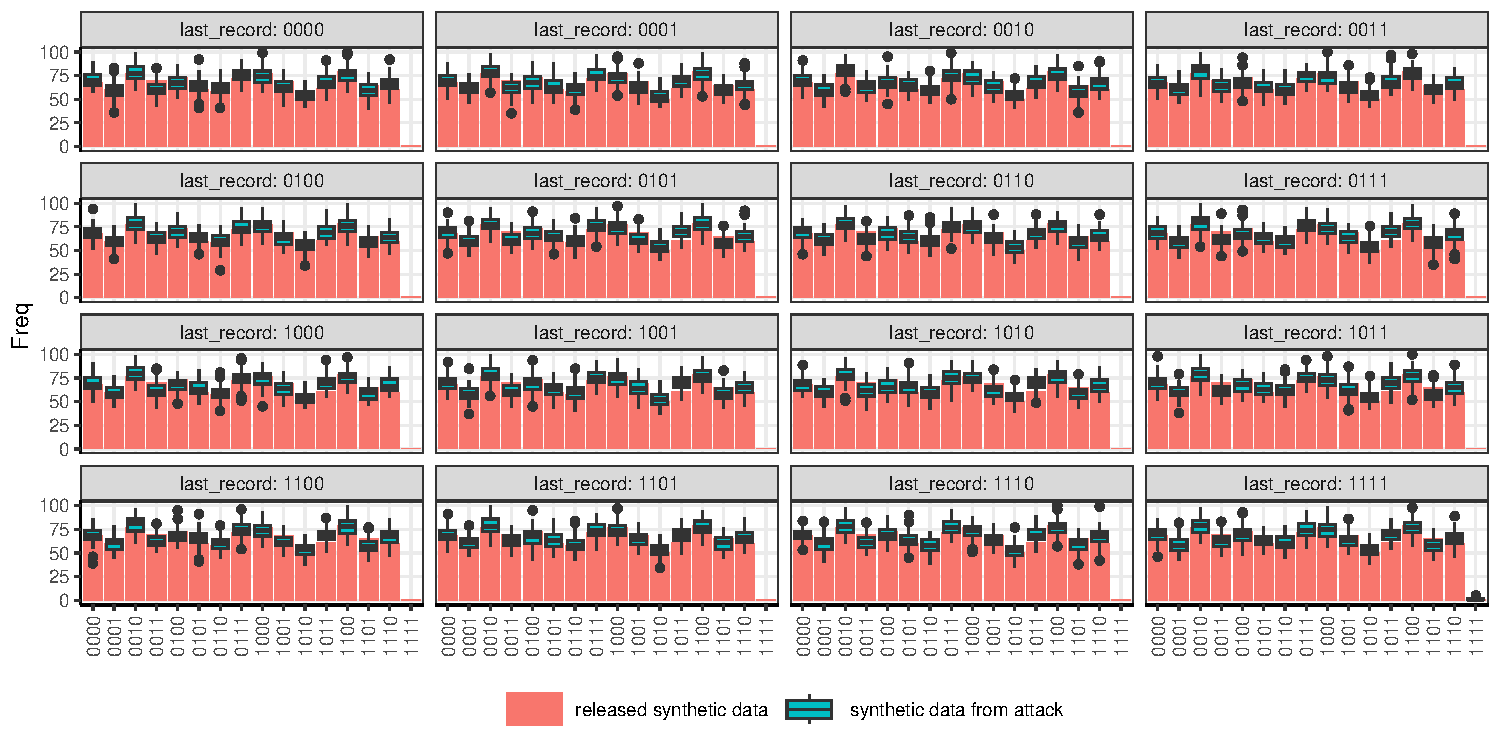
\includegraphics{../graphs/graph_attacker_default.pdf}}
    \label{fig:attacker_default}
\end{figure}

If the attacker guesses that the last record is 0,0,0,0, then they are not able to replicate the single unique record in the synthetic data.  As stated earlier, the reason is that a record may not be in the synthetic data if it is in the original data, but it can only be in the synthetic data if it is also in the original data. 

Next, they update their beliefs about the last record and guess that the last record in the original data is 0,0,0,1.  They then repeat the process as described above.  This is shown in the top row, second column from the left.  Like their first guess, they cannot replicate the released synthetic data.  

The attacker then repeats this process for all 16 possible combinations of the last record.  Finally, if they guess that the last record is 1,1,1,1, then they are able to replicate the released synthetic data, as shown in the bottom, right cell.  The result is a successful attack with confirmation that guess about the values of the last, unique observation is correct.

\section{Disclosure risk measures}

Our results show that CART can produce synthetic data that is disclosive because it replicates unique records from the original data set without adding sufficient noise.  By itself, this is not a problem.  However, this is a problem if we are not able to measure this disclosure.  The literature on privacy measures for synthetic data is well-developed \cite{wagner2018technical}.  One reason why there are so many measures of privacy is because there is no one agreed upon understanding of either what defines risk nor how one should measure it.  

We use three commonly understood measures of privacy implemented by the Synthpop package in R \cite{raab2024practical,elliot_etal_2020,raab2024practical}, each with its own strengths and weaknesses. Identity disclosure refers to the ability to identify individuals in the data from a set of known characteristics, i.e. `keys'. Specifically, it measures the percent of all records in the data for which the keys identify a unique record in the synthetic data ($UiS$) and in the original data ($UiO$).  The authors of Synthpop recommend $repU$ (replicated uniques) to measure identity disclosure as the percent of unique records in original data ($UiO$) that are also unique in the synthetic data ($UiS$).  One advantage is an easy to understand measure of privacy risks.  One disadvantage is that the results are sensitive to the choice of key variables and the improper selection of keys may over or underestimate privacy risks.

Attribute disclosure refers to the ability to identify a previously unknown characteristic of an individual.  Synthetic data are SD and original data are ground truth (GT).  In this approach, an attacker who wants to infer a sensitive attribute ($t$), has access to SD, and knows one or more identifiers in the GT ($q$, i.e. composite keys, as in above).  The measure is derived in the following way: (i) in synthetic ($iS$) is the proportion of all records for a given $q$ in the GT with the same $q$ in the SD; (ii) disclosive in synthetic ($DiS$) is the proportion of all $iS$ who also have the same $t$; (iii) disclosive in synthetic correct in original ($DiSCO$) is the proportion of $DiS$ that match the original value of $t$ in the GT.  $DiSCO$ is compared to disclosive in original ($Dorig$) or the proportion of all records where the keys would identify a unique value of the target in the GT.  The measure of attribute disclosure shares similar advantages and disadvantages with identity disclosure.

Finally, replicated uniques ($repU$) assess privacy risk by identifying records in the dataset that are unique and thus more vulnerable to re-identification, particularly when matched with external data sources. The advantage is that it is both easy to understand and effective in highlighting records most at risk (i.e. uniques).  The disadvantage is it may oversimplify privacy risks by focusing only on uniqueness while neglecting broader contextual factors like record-linkage or attribute disclosure.  However, by considering these three measures, we aim to provide a balanced evaluation of privacy risks while acknowledging their distinct advantages and limitations.  

We apply these measures to the original and synthetic data from figure \ref{fig:compare}, as shown in table \ref{table:disclosure_risk}.  The keys are the first 3 binary variables ($q$) and the target or sensitive attribute is the last binary variable ($t$).For reference, we replicated table \ref{table:disclosure_risk} with 100 synthetic copies from figure \ref{fig:cart_histogram_compare_100}, as shown in table \ref{table:disclosure_risk_100} in the Appendix.  Results are qualitatively similar.  

\begin{table}[]
    \centering
    \caption{Disclosure risk measures}
    \begin{tabular}{llll}
        \toprule
        Privacy   & Identity & Attribute & Uniques \\ \midrule
        Original  & 0\%      & 0\%       & 0.1\% (1) \\
        Synthetic & 0\%      & 0\%       & 0.1\% (1) \\ 
        \bottomrule
    \end{tabular}
    \label{table:disclosure_risk}
\end{table}

In the first column, we display the identity disclosure risk based on the keys for the original and synthetic data, as shown in the first and second row, respectively.  The measure indicates that these three variables cannot identify any unique observations in either the original or synthetic data.  This is correct because we know that there are multiple combinations of var1=(0,1),var2=(0,1),var3=(0,1).  

In the second column, we display the attribute disclosure risk based on the ability to uniquely identify the $t$ from $q$ in the original and synthetic data.  According to this measure, there is no risk of attribute disclosure in the original or synthetic data.  This is a not correct because we know that when $q=111$, there is a unique record of $t=1$.  

In the third column, we display the uniques, there are 0.1\% (1/1000) in the original and synthetic data.  This would signal a cause for concern because the synthetic data perfectly replicates the number of uniques in the original data.  At first, it might appear that the solution would be to simply reduce another synthetic data set with a different seed or even multiple synthetic data sets.  However, even if one released 100 synthetic data sets, as shown in figure \ref{fig:cart_histogram_compare_100}, one might solve the problem of replicated uniques as values of 1,1,1,1 would range from 0 to 3 (as described earlier), but this would not solve the problem of disclosure.  

In summary, the only privacy measure that would indicate there is a problem with disclosure risk in the original or synthetic data is the number of unique records in both.  In short, the main issue of concern is that we know there is a disclosure problem (because we created it), but the disclosure risk measures commonly used in the literature do not capture the problem.  

The good news.  We can correct the problem of disclosure risk in synthetic data generated from CART-based SDGs.  If we modify the parameters to prevent overfitting, then the disclosure problem goes away.  Multiple options exist to do this.  We use two: increase the minimum number of observations per terminal node to 75 (default is 5) and increase the complexity parameter to 0.05 (default is 1e$^{-8}$), as shown in figure \ref{fig:compare_modified}.  These adjustments clearly reduce disclosure risks.

\begin{figure}[!h]
    \centering
    \caption{Compare original and synthetic data}
    \begin{subfigure}{0.48\textwidth}
        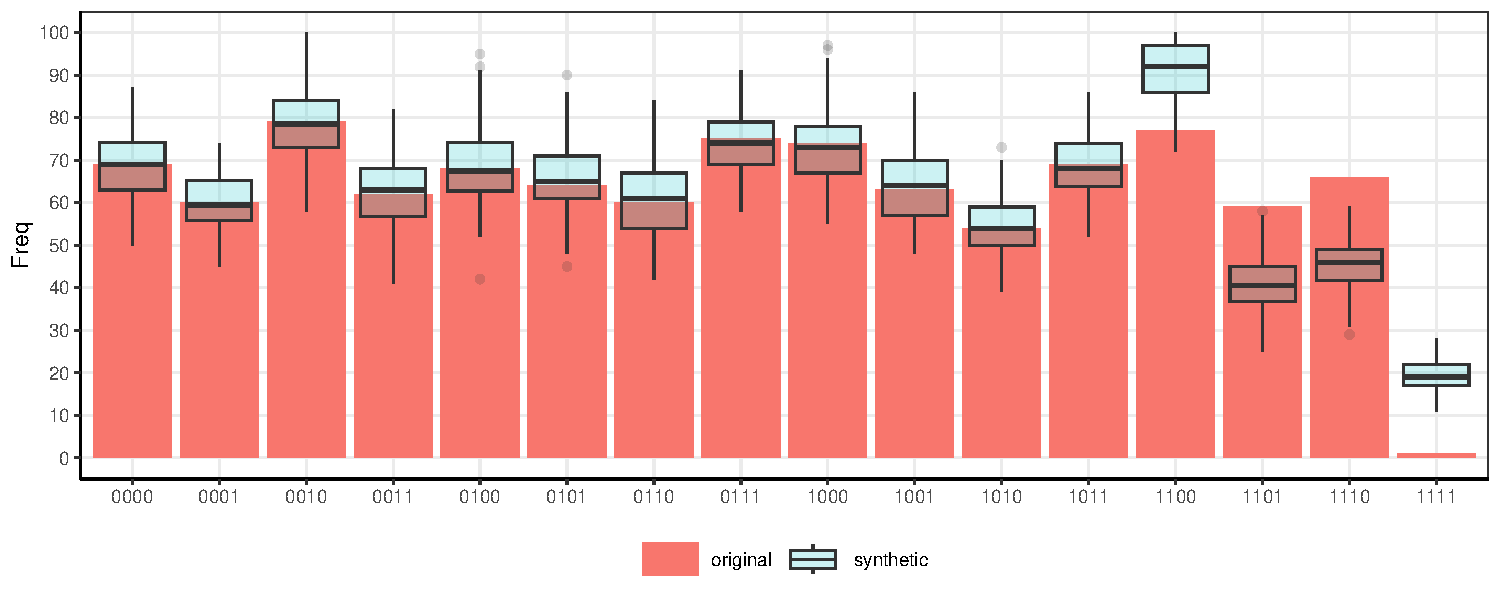
\includegraphics[width=\textwidth]{../graphs/graph_cart_modified_mb_histogram_compare_100.pdf}
        \caption{Minimum bucket is 75}
        \label{fig:attacker_modified_mb}
    \end{subfigure}
    \hfill
    \begin{subfigure}{0.48\textwidth}
        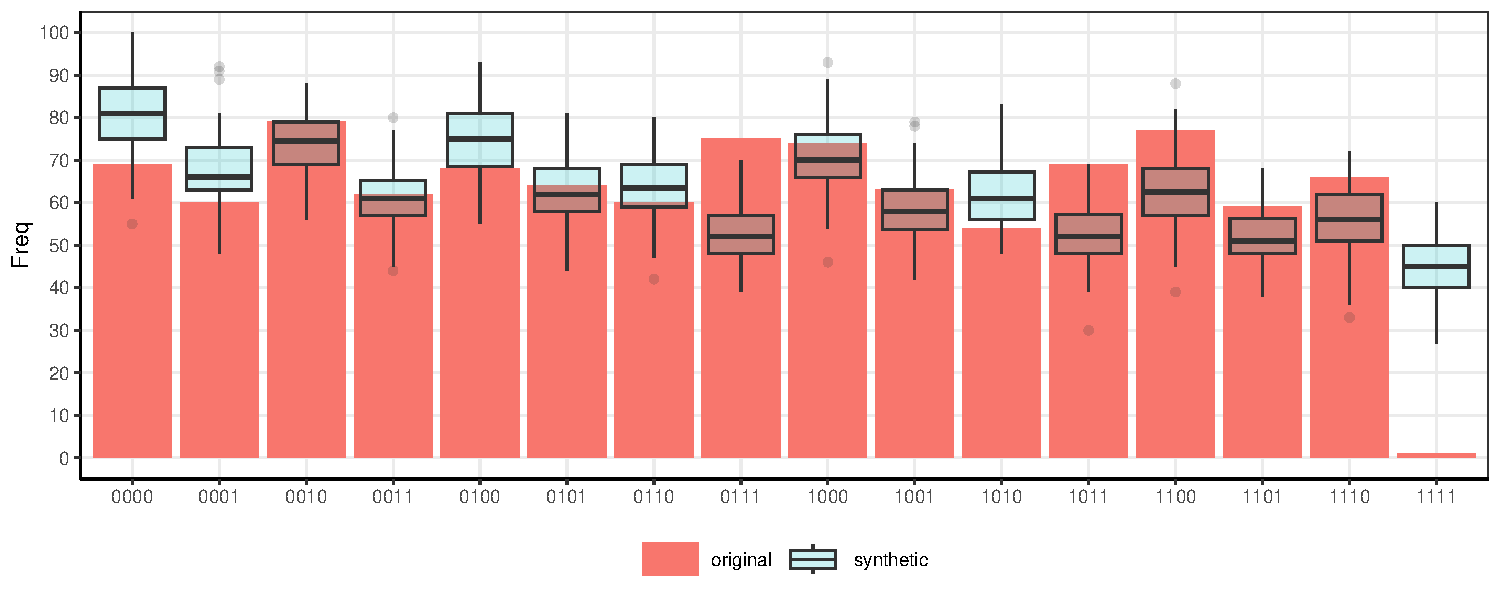
\includegraphics[width=\textwidth]{../graphs/graph_cart_modified_cp_histogram_compare_100.pdf}
        \caption{Complexity parameter is 0.05}
        \label{fig:attacker_modified_cp}
    \end{subfigure}
    \label{fig:compare_modified}
\end{figure}

The bad news.  First, the modified synthetic data may increase privacy, but the sacrifice is lower utility.  Even with 100 synthetic data sets, figure \ref{fig:compare_modified} is less representative of the original data set than \ref{fig:cart_histogram_compare_100}.  Second, in an important way, we are choosing to decrease utility in order to increase privacy.  Remember, as we have shown, no commonly used disclosure risk measure indicates that there is a problem.  In a real world example, this would raise the question of whether such sacrifices are justified when risks are not apparent.

\section{Discussion}


4.1 The Utility-Privacy Trade-Off

Our findings confirm the long-held understanding of a utility-privacy trade-off in synthetic data generation. CART models, despite their perceived robustness, are not immune to this trade-off.

4.2 Limitations of Current Privacy Metrics

The inability of common metrics to capture disclosure risks highlights the need for enhanced evaluation tools. Relying on these metrics alone may result in an underestimation of privacy vulnerabilities.

4.3 Implications for Practice

The results emphasize the need for cautious use of CART-based SDGs, particularly when handling datasets with unique records. Practitioners should consider:

    •   Implementing robust parameter tuning to mitigate risks.
    •   Combining CART with other privacy-preserving techniques.
    •   Developing new metrics to capture nuanced risks.

\section{Conclusion}

This study demonstrates that CART-based SDGs are susceptible to privacy risks, particularly in scenarios involving unique records. While parameter adjustments can enhance privacy, they necessitate a reduction in utility. Importantly, common privacy metrics failed to detect these risks, underscoring the limitations of existing tools.

Key Takeaways

    1.  CART-based models are not inherently immune to the utility-privacy trade-off.
    2.  Common privacy metrics may fail to detect significant risks.
    3.  Sacrificing utility is often necessary, but only if risks are known in advance.


\begin{credits}
\subsubsection{\ackname} This work was supported by a grant from the German Federal Ministry of Education and Research (grant number 16KISA096) with funding from the European Union—NextGenerationEU.  Reproducible files are located here: \url{https://github.com/jonlatner/KEM\_GAN/tree/main/latner/projects/simulation}

\subsubsection{\discintname}
The authors have no competing interests to declare that are relevant to the content of this article.
\end{credits}


%%%%%%%%%%%%%%%%%%%%%%%%%%%%%%%%
% Bibliography
%%%%%%%%%%%%%%%%%%%%%%%%%%%%%%%%
\bibliographystyle{splncs04}
\bibliography{references}

%%%%%%%%%%%%%%%%%%%%%%%%%%%%%%%%
% Appendix
%%%%%%%%%%%%%%%%%%%%%%%%%%%%%%%%
\clearpage
\appendix
\section{Appendix}\label{appendix}
\setcounter{figure}{0}    
\setcounter{table}{0}    
\renewcommand*\thetable{\Alph{section}.\arabic{table}}
\renewcommand*\thefigure{\Alph{section}.\arabic{figure}}
\renewcommand{\theHfigure}{\Alph{section}.\arabic{table}}
\renewcommand{\theHtable}{\Alph{section}.\arabic{figure}}

\begin{table}[]
    \centering
    \caption{Disclosure risk measures from 100 synthetic data sets}
    \begin{tabular}{llll}
        \toprule
        Privacy   & Identity & Attribute & Uniques \\ \midrule
        Original  & 0\%      & 0\%       & 0.1\% (1/1000) \\
        Synthetic & 0\%      & 2.51\%       & 0.29\% (29/100)  \\ 
        \bottomrule
    \end{tabular}
    \label{table:disclosure_risk_100}
    \vspace{0.5em} % Add some space between the table and the note
    \noindent\parbox{0.8\textwidth}{\footnotesize  Note: In the uniques from original data, there is 1 unique observation out of 1000.  In the uniques from 100 synthetic data sets, 29 out of 100 data sets replicate 1 unique for 1,1,1,1. The other synthetic data sets have between 0 and 3 records for 1,1,1,1.}
\end{table}

\clearpage
\begin{table}[]
    \centering
    \caption{Frequency from 5 synthetic data sets}
    \begin{tabular}{llllll}
        \toprule
        combine & 1 & 2 & 3 & 4 & 5 \\ \midrule
        0000 & 68 & 73 & 61 & 83 & 76 \\
        0001 & 60 & 63 & 66 & 58 & 66 \\
        0010 & 77 & 78 & 80 & 68 & 90 \\
        0011 & 70 & 63 & 53 & 60 & 55 \\
        0100 & 73 & 55 & 67 & 63 & 64 \\
        0101 & 60 & 59 & 71 & 63 & 68 \\
        0110 & 58 & 62 & 56 & 54 & 52 \\
        0111 & 72 & 89 & 61 & 87 & 68 \\
        1000 & 77 & 76 & 84 & 65 & 66 \\
        1001 & 69 & 67 & 71 & 69 & 72 \\
        1010 & 50 & 60 & 54 & 64 & 52 \\
        1011 & 61 & 60 & 71 & 62 & 76 \\
        1100 & 79 & 78 & 84 & 79 & 79 \\
        1101 & 65 & 58 & 56 & 55 & 59 \\
        1110 & 60 & 57 & 64 & 69 & 57 \\
        1111 & 1  & 2  & 1  & 1  & 0  \\
        \bottomrule
    \end{tabular}
    \label{table:frequency_5_data_sets}
\end{table}


\begin{table}[]
    \centering
    \caption{Attribute risk measures from 5 synthetic data sets}
    \begin{tabular}{lllllll}
        \toprule
            m &   Dorig & Dsyn & iS & DiS & DiSCO & DiSDiO \\ \midrule
            1 &    0 &  0.0 & 100 & 0.0 &   0.0 &      0 \\
            2 &     0 &  0.0 & 100 & 0.0 &   0.0 &      0 \\
            3 &     0 &  0.0 & 100 & 0.0 &   0.0 &      0 \\
            4 &     0 &  0.0 & 100 & 0.0 &   0.0 &      0 \\ 
            5 &     0 &  5.7 & 100 & 6.7 &   6.6 &      0 \\ 
        \bottomrule
    \end{tabular}
    \label{table:attribute_disclosure_risk_5}
    \vspace{0.5em} % Add some space between the table and the note
    \noindent\parbox{0.8\textwidth}{\footnotesize Note: t1\$output.list\$var4\$attrib}
\end{table}

\end{document}
